\documentclass[12pt,a4paper]{report}  % ←ドキュメントクラスを追加
\usepackage[utf8]{inputenc}           % 文字コード指定
\usepackage{geometry}                 % 余白調整
\geometry{left=15mm,right=15mm,top=15mm,bottom=15mm}
\usepackage{url}

\usepackage{setspace}                 % 行間調整用
\usepackage{amsmath,amssymb}          % 数式用
% \usepackage{graphicx}                 % 画像を使う場合
\usepackage{titlesec}         
\usepackage[dvipdfmx]{graphicx} % 画像を使うためのパッケージ(日本語環境ならこれが無難)
\usepackage{here}          % 章タイトル調整
\usepackage{caption} % プリアンブルで追加
\renewcommand{\figurename}{図}
\renewcommand{\tablename}{表}

% --- 独自コマンド ---
\newcommand{\divergence}{\mathrm{div}\,}  % ダイバージェンス
\newcommand{\grad}{\mathrm{grad}\,}       % グラディエント
\newcommand{\rot}{\mathrm{rot}\,}         % ローテーション

% --- ページスタイル ---
\pagestyle{myheadings}

% --- タイトル情報 ---
\title{\Huge システムプログラミングII\\最終レポート}
\author{学生番号:5428 \\ 氏名:堀川風花}
\date{提出日:2025年1月21日}

\begin{document}

\maketitle    % ← タイトル(表紙)をここで出力!

% \setstretch{1.5}  % 行間を1.5倍に設定

\noindent
% レポート課題(11/11提出)\\[1em]  % ← [1em] は改行後の余白
\section{はじめに}
\subsubsection{目的}
\subsubsection{背景}

\section{サービスの概要}
本レポートでは以下のような構成のレンタルスペースの予約サービス(以下、本サービスという)を開発する。
本サービスでは会議室やパーティルームなどの「レンタルスペース」を、ユーザーがオンラインで予約できるサービスである。
管理者はレンタルスペースの登録や予約状況の確認などができる。
またレンタルスペースを予約した利用者は利用開始時刻の1時間前にGmailでリマインダーを受信する。

\begin{itemize}
  \item ユーザーの管理(認証、識別) \mbox{}\\
  本サービスを利用するユーザーを識別し、操作するための機能である。
  複数人でサービスを利用するため、ユーザーを追加したり、利用ユーザーを識別する機能が必要となる。
  \item レンタルスペースの管理(削除、編集、登録)\mbox{}\\
  レンタルスペースを予約する際には、まず予約する対象であるレンタルスペースを管理する必要がある。
  そのレンタルスペースの追加、削除できるようにする。
  \item レンタルスペースの予約の管理(キャンセル) 
  誰がそのレンタルスペースの予約をしているのかを管理する。
  \item リマインダー(Gmailに送信)
  利用開始時刻の1時間前に利用者のメールアドレスにGmailでリマインダーや
  サービスを提供できなくなった場合のキャンセルメール、
  利用が終了した際の感謝メールを送信する。
\end{itemize}


\section{システム構成}
\begin{center}
  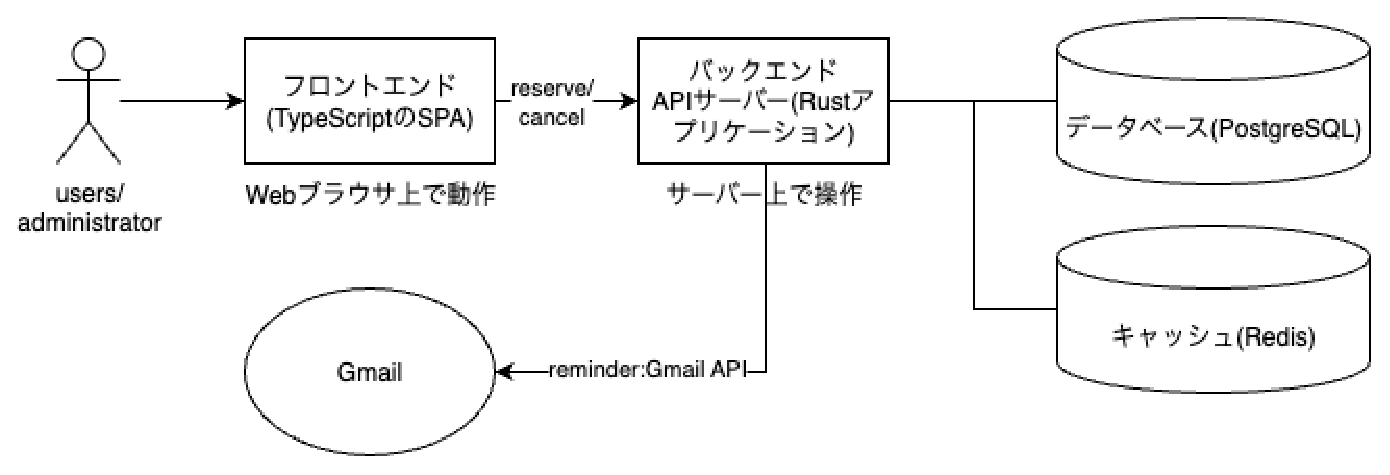
\includegraphics[width=0.7\linewidth]{/Users/horikawafuka2/Documents/class_2025/sp/reports/images/service2.eps}
  \captionof{figure}{サービス概要図}
  \label{fig:system_image}
\end{center}

\subsection{使用技術}
\begin{table}[h]
  \centering
\begin{tabular}{|l|r|} \hline
   分類& 使用技術  \\ \hline
   フロントエンド & TypeScript、React(Next.js) \\ \hline
   データベース &  PostgreSQL\\ \hline
   キャッシュ & Redis  \\ \hline
   バックエンド & Rust  \\ \hline
   サーバ & docker \\ \hline
   リマインダー & Gmail API\\ \hline
 \end{tabular}
   \caption{使用技術}
  \label{tb:use_module}
\end{table}

\subsection{モジュール構成}




\section{データベース設計}

データベース設計は図 \ref{fig:database_image}の通りである。

\begin{table}[h]
  \centering
\begin{tabular}{|l|r|} \hline
   データベース名& 内容  \\ \hline
   roles & \\ \hline
   users &  PostgreSQL\\ \hline
   spaces & Redis  \\ \hline
   resrvations & Rust  \\ \hline
   returned\_reservations & docker \\ \hline
 \end{tabular}
   \caption{使用技術}
  \label{tb:use_module}
\end{table}
\begin{center}
  \includegraphics[width=0.4\linewidth]{/Users/horikawafuka2/Documents/class_2025/sp/reports/images/database.eps}
  \captionof{figure}{データベース図}
  \label{fig:database_image}
\end{center}

\section{各種機能}
\subsection{利用者向け機能}
\subsubsection{予約機能}
\subsubsection{予約確認機能}
\subsection{管理者向け機能}
\subsubsection{予約一覧表示機能}
\subsubsection{管理操作機能}

\subsection{通知機能}
\subsubsection{リマインドメール送信機能}
\subsubsection{キャンセルメール送信機能}


\subsection{加点対象機能}
\subsubsection{感謝メール送信機能}

\section{動作確認}
\subsection{動作確認環境}
\subsection{利用者操作の動作確認手順}
\subsection{管理者操作の動作確認手順}

\section{振り返り}
\section{まとめ}

\vskip\baselineskip











\vskip\baselineskip

\subsubsection{グループの傾向}
\begin{itemize}
\item グループ1 \mbox{}\\
複数のトピックが共通しており、トピックの内容は地域や教育関係と
広い範囲にわたる。地域行政や学校教育を重視する傾向がある。

\item グループ2 \mbox{}\\
教育・学校・教育\_委員などの教育行政のトピックが強いエッジで重なっており、
教育関係と教育を受ける子供を重視する傾向がある。 
\item グループ3 \mbox{}\\
発電・エネルギー・電力などインフラ関係やエネルギー政策に関心があることが見てとれる。
  \end{itemize}

\vskip\baselineskip



% \begin{center}
%   \includegraphics[width=0.7\linewidth]{/Users/horikawafuka2/Documents/class_2025/dm/後期中間/reports/images/700_speakers_cc_network_colored.eps}
%   \captionof{figure}{グループ分けした共起ネットワーク(議員24人)}
% \end{center}


\section{参考文献}
% 参考文献を強制改ページしない設定
\begingroup
\renewcommand{\chapter}[2]{} % chapterとして認識させない
\begin{thebibliography}{2}
\bibitem{word cloud} Non."【簡単】Pythonでワードクラウドを作る方法".note.20243-09-13,\url{https://note.com/noa813/n/n777ba133e62f},(2025-10-28)
\bibitem{cc network} osn Lofi."【自然言語処理】【Python】共起ネットワークの作り方を理解する".Zenn.2022-10-08,\url{https://zenn.dev/robes/articles/a3e1a6e80efd99},(2025-10-29)
\bibitem{masuzoe yoichi} 公明党."都市外交を積極的に".公明党公式ホームページ.2014-03-05,\url{https://www.komei.or.jp/news/detail/20140305_13423},(2025-11-03)

\end{thebibliography}
\endgroup

\end{document}